% PRL look and style (easy on the eyes)
\documentclass[aps,pre,twocolumn,nofootinbib,superscriptaddress,linenumbers]{revtex4-1}
% Two-column style (for submission/review/editing)
%\documentclass[aps,prl,preprint,nofootinbib,superscriptaddress,linenumbers]{revtex4-1}

\pdfoutput=1
\usepackage[pdftex]{graphicx}

\usepackage{alltt}

%\usepackage{palatino}

%\usepackage{palatino}
% Change to a sans serif font.
\usepackage{sourcesanspro}
\renewcommand*\familydefault{\sfdefault} %% Only if the base font of the document is to be sans serif
\usepackage[T1]{fontenc}
%\usepackage[font=sf,justification=justified]{caption}
\usepackage[font=sf]{floatrow}

% Rework captions to use sans serif font.
\makeatletter
\renewcommand\@make@capt@title[2]{%
 \@ifx@empty\float@link{\@firstofone}{\expandafter\href\expandafter{\float@link}}%
  {\sf\textbf{#1}}\sf\@caption@fignum@sep#2\quad
}%
\makeatother

\usepackage{listings} % For code examples
\usepackage[usenames,dvipsnames,svgnames,table]{xcolor}

\usepackage{amsmath}
\usepackage{amssymb}
%\usepackage[mathbf,mathcal]{euler}
%\usepackage{citesort}
\usepackage[caption=false]{subfig}
\usepackage{dcolumn}
\usepackage{boxedminipage}
\usepackage{verbatim}
\usepackage[colorlinks=true,citecolor=blue,linkcolor=blue]{hyperref}
\usepackage[group-separator={,}]{siunitx}

%Strikethrough
\usepackage{ulem}

% Justification
\captionsetup{singlelinecheck=off}

% Pretty-printing of shell commands
\newcommand{\shellcmd}[1]{\\\ \texttt{\scriptsize #1}}

% The figures are in a figures/ subdirectory.
\graphicspath{{../figures/}}

%% DOCUMENT %%%%%%%%%%%%%%%%%%%%%%%%%%%%%%%%%%%%%%%%%%%%%%%%%%%%%%%%%%%%%%%%%%%%
\begin{document}

%% TITLE %%%%%%%%%%%%%%%%%%%%%%%%%%%%%%%%%%%%%%%%%%%%%%%%%%%%%%%%%%%%%%%%%%%%
\title{Modeling experimental error in assays:\\
Understanding discrepancies between assays using different dispensing technologies}

\author{Sonya M. Hanson}
  \affiliation{Computational Biology Program, Sloan Kettering Institute, Memorial Sloan Kettering Cancer Center, New York, NY 10065, United States}
\author{Sean Ekins}
  \affiliation{Collaborations in Chemistry, Fuquay-Varina, NC 27526, United States}
\author{John D. Chodera}
 \thanks{Corresponding author}
 \email{john.chodera@choderalab.org}
  \affiliation{Computational Biology Program, Sloan Kettering Institute, Memorial Sloan Kettering Cancer Center, New York, NY 10065, United States}

\date{\today}

%%%%%%%%%%%%%%%%%%%%%%%%%%%%%%%%%%%%%%%%%%%%%%%%%%%%%%%%%%%%%%%%%%%%%%%%%%%%%%%%%%%%%%%%%%%%%%%%%%%%%%
% ABSTRACT/pacs
%%%%%%%%%%%%%%%%%%%%%%%%%%%%%%%%%%%%%%%%%%%%%%%%%%%%%%%%%%%%%%%%%%%%%%%%%%%%%%%%%%%%%%%%%%%%%%%%%%%%%%
\begin{abstract}

All experimental assay data contains error, but understanding the magnitude, type, and primary origin of this error is not often obvious.
Here, we describe a simple set of assay modeling techniques based on the bootstrap principle that allow sources of error and bias to be simulated and propagated into assay results.
We demonstrate how deceptively simple operations---such as the creation of a dilution series with a robotic liquid handler---can significantly amplify imprecision and even contribute substantially to bias.
To illustrate these techniques, we review an infamous example of how choice of dispensing technology greatly impacted assay measurements, and show how the primary contributions to discrepancies between assays can be easily understood and potentially corrected for.
These simple modeling techniques---illustrated with an accompanying IPython notebook---can allow modelers to understand the expected error and bias in experimental datasets, and even help experimentalists design assays to more effectively reach accuracy and imprecision goals.

\end{abstract}

\maketitle

%%%%%%%%%%%%%%%%%%%%%%%%%%%%%%%%%%%%%%%%%%%%%%%%%%%%%%%%%%%%%%%%%%%%%%%%%%%%%%%%%%%%%%%%%%%%%%%%%%%%%%
% INTRODUCTION
%%%%%%%%%%%%%%%%%%%%%%%%%%%%%%%%%%%%%%%%%%%%%%%%%%%%%%%%%%%%%%%%%%%%%%%%%%%%%%%%%%%%%%%%%%%%%%%%%%%%%%
\section{Introduction}
\label{section:introduction}

Measuring the activity and potency of ligands---whether in biophysical or cell-based assays---is a critical tool in the understanding of biological processes.
However, understanding assay data for the purpose of optimizing small molecules for use as chemical probes or potential therapeutics is complicated by the fact that all assay data are contaminated with error from numerous sources.

Often, the dominant contributions to assay error are simply not known.
This is unsurprising, given the number and variety of potential contributing factors.
Even for what might be considered a straightforward assay involving fluorescent measurements of a ligand binding to a protein target, this might include (but is by no means limited to): compound impurities and degradation~\cite{kozikowski_effect_2003,kozikowski_effect_2003-1,cheng_studies_2003,waybright_overcoming_2009}, imprecise compound dispensing {\color{red}[CITE?]}, unmonitored water absorption by DMSO stocks {\color{red}[CITE?]}, the effect of DMSO on protein stability~\cite{tjernberg_dmso-related_2005}, intrinsic compound fluorescence~\cite{simeonov_fluorescence_2008,baell_new_2010}, compound insolubility~\cite{di_biological_2006} or aggregation~\cite{mcgovern_common_2002,mcgovern_kinase_2003,feng_high-throughput_2005,feng_synergy_2006,baell_new_2010}, variability in protein concentration or quality, pipetting errors, and inherent noise in any fluorescence measurement---not to mention stray lab coat fibers as fluorescent contaminants~\cite{busch_does_2015}. 
In an ideal world, control experiments would be performed to measure the magnitude of these effects, and data quality tests would either reject flawed data or ensure that all contributions to error have been carefully accounted for in producing an assessment of error and confidence for each assayed value.

%Often computational chemists are faced with comparing their models to experimental assay data for which there is no clear idea of the magnitude of the error. Sometimes no error is provided. Sometimes only a ballpark estimate is given. It would be useful to be able to get an estimate of how confident one should be in the data they are looking at. Other times, one might want to ensure ahead of time that an assay will produce useful data. For example if the error is larger than the dynamic range of the expected measurements, the assay will not be very useful.

Unfortunately, by the time the data reach the hands of a modeler (or other data consumer), the opportunity to perform these careful control experiments has passed.
In the worst case, the communicated assay data may not contain any estimate of error at all. Even when error has been estimated, it is often not based on a holistic picture of specific information known about the assay.
One approach that has been useful is aggregating many datasets to give a crude estimate of the general reliability of a similar set of assays by quantifying the variation in measurements of a single quantity~\cite{kramer_experimental_2012,kalliokoski_comparability_2013}. 
Care must be taken to distinguish between fully independent replicates and partial replicates that only repeat part of the experiment (for example, repeated measurements performed using the same stock solutions), since partial measurements can often underestimate true error by orders of magnitude~\cite{jdc-itc-paper}.
Alternatively, when multiple independent measurements are not available, the knowledge of how a particular assay was conducted can inform the construction of an assay-specific model incorporating some of the dominant contributions to error in a manner that can be highly informative.

%In many papers and reports errors or not provided or are inadequately explained. Our understanding of the reliability of experimental measurements of ligand binding affinity would be greatly increased if it was common practice to calculate expected experimental errors resulting from the major known sources.

In this paper, we review some common sources of error in experimental assays, and describe some simple modeling tools based on the bootstrap principle for simulating a model of an assay that incorporates these important (often dominant) sources of error. 
This approach, while simple, provides a powerful tool to understand how assay error depends on  known parameters. 
For example, with this approach, we can estimate the expected data error as a function of true compound affinity.
Not only modelers could benefit from this approach---these tools can be also used to help optimize assay formats before an experiment is performed, help troubleshoot problematic assays after the fact, or ensure that all major sources of error accounted for by checking that variations among controls match expectations.

We illustrate these concepts by considering a now-infamous example from the literature: a report by Ekins et al.~\cite{ekins_dispensing_2013} on how the choice of dispensing technology impacts the apparent biological activity of the same set of compounds under otherwise identical conditions.
The datasets employed in the analyses {\color{red}[CITE]} were generated using either a standard liquid handler with fixed (washable) tips\footnote{{\color{red}We should have a footnote clarifying how we know these were fixed tips.}} or an acoustic droplet dispensing device to prepare the assay, resulting in highly divergent assay results (Figure~\ref{fig:overview}).
While the frustration for modelers was particularly great, since QSAR models derived from these otherwise identical assays produce surprisingly divergent predictions, numerous practitioners from all corners of drug discovery expressed their frustration in ensuing blog posts and commentaries~\cite{in-the-pipeline-comments}.
Hosts of potential reasons were speculated~\cite{in-the-pipeline-comments}, including [LIST HERE].

We make use of this real-world example to illustrate some of the basic concepts behind modeling the most common sources of error in assays.
For simplicity, we ask whether the most basic contributions to assay error---imprecision and bias in material transfer operations and imprecision in measurement---might account for some component of the discrepancy between assay techniques.
We make use of basic information---the assay protocol as described (with some additional inferences based on basic concepts such as compound solubility limits) and manufacturer specifications for imprecision and bias---to construct a model of each dispensing process to determine the overall inaccuracy and imprecision of the assay as a function of true compound affinity, and identify the steps that contribute the most to these assay data errors.
To better illustrate these techniques, we also provide an annotated IPython notebook that includes all of the computations described here in detail.
Readers are encouraged to download these notebooks and play with them to see how different assay configurations affect assay error.

\begin{figure*}[tb]
   \includegraphics[trim={0 15cm 0 8cm},clip,width=0.75\textwidth]{../figures/Fig1-3.pdf}
  \caption{{\bf The stages of creating a dilution series with either tip-based or acoustic dispensing.}
  On the way from the raw material to the assay measurement there are a variety of steps. 
  In the case of tip-based dispensing, such as for the Tecan Genesis, an initial dilution of ligand stock into buffer is created and then serially diluted to create the full dilution series used in the final detection and construction of saturation curves. 
  In the case of acoustic dispensing, such as for the LabCyte Echo, the full dilution series is made via direct dispensing, which has a uniform error at each stage of the dilution.
  }
  \label{fig:overview}
\end{figure*}


%%%%%%%%%%%%%%%%%%%%%%%%%%%%%%%%%%%%%%%%%%%%%%%%%%%%%%%%%%%%%%%%%%%%%%%%%%%%%%%%%%%%%%%%%%%%%%%%%%%%%
% Experimental error
%%%%%%%%%%%%%%%%%%%%%%%%%%%%%%%%%%%%%%%%%%%%%%%%%%%%%%%%%%%%%%%%%%%%%%%%%%%%%%%%%%%%%%%%%%%%%%%%%%%%%
\section{Experimental error}

Overall experimental error can be broken into two components: The \emph{imprecision} (or variance), which characterizes the random component of the error that causes different replicates of the same assay to give slightly different results, and the \emph{inaccuracy} (or bias), which is the deviation of the average over many replicates from the true value of the quantity being measured.

There are a variety of sources of experimental error. 
For imprecision, random variation in the quantity delivered by a pipette, random errors in the reported mass of a dry compound, or random errors in the measured fluorescence of a well will all contribute. 
The important thing is that the mean of these errors over many repetitions is zero. 
If the mean is \emph{not} zero, this is an example of inaccuracy, or bias---where a calibration error leads to a systematic deviation in the volume delivered by a pipette, the mass measured by a balance, or the average fluorescence measured by a plate reader.

\section*{Modeling experimental error}

Modeling experimental error can be done in many ways. 
Here we take the approach that it is as simple as adding known values for imprecision and inaccuracy in pipetting into a model of your assay, and using parametric bootstrapping [ref] to sample through many replicates and getting a resulting expected bias and coefficient of variation (CV), which correspond to the imprecision and inaccuracy, respectively. 

Since the main values for imprecision and inaccuracy that we need to consider are those for the volumes being pipetted, to sample across many replicates we just randomly draw from a normal distribution:
\begin{equation} \label{eq:1}
Volume \sim \mathcal{N}(\mu,\sigma^2) 
\end{equation}
where $\mu$ is the bias and $\sigma^2$ is the variance, which are defined by the imprecision and inaccuracy values, respectively, provided by the manufacturer of the liquid-handler.

\subsection*{Error propagation}

Error propagation, for example when we have many pipetting steps in a row each with its own error, can be a bit trickier to implement. 
While there are a variety of ways of doing this, derivable from the Taylor Expansion, using parametric bootstrapping [ref] to sample through many replicates, as mentioned above, avoids having to implement these more complex forms of error propagation.
Bootstrapping allows you to approximate the sampling distribution by simulating from a good estimate of the real process.
The more common form of boostrapping is resampling bootstrapping, where the 'good estimate of the real process' resamples estimates from the observed sample.
Here, parametric bootstrapping is used, where the 'good estimate of the real process' is a simulation of a model.
This works well for a variety of models, and here we show it for a specific rather simple case, but it can be expanded to include much more complicated error models, without making the math of the error propagation any more complicated.
In this case knowing the sampling distribution lets us quantify uncertainty

\subsection*{Simple liquid handling: Mixing solutions}

When an assay involves mixing two compounds together, as with most assays, you also have to consider mixing efficiency. 
For example if an assay involves mixing compound stock with a protein solution, usually a small volume into a much larger volume, uneven mixing can cause wide variation in the results. 
\begin{itemize}
  \item Several examples of this have been seen [ref,ref]
  \item Mention that the difficulties in mixing are not even considered in our simple model (we just assume good mixing).
\end{itemize}

\subsection*{Making a dilution series}

Dilution series are often used to characterize the activity and potency of ligands. 
In dilution series, error propagation is especially important, as pipetting happens as many times as there are steps in the dilution, with each pipetting step contributing its own error. 
Thus, the instrumentation used can have a real effect on the results obtained.
Here we compare an aqueous dilution series made with a tip-based liquid handler (specifically the Tecan Genesis), and a direct-dispensing dilution series made with acoustic dispensing (specifically the Labcyte Echo).

\subsubsection*{Tip-based liquid handling.}

To construct a model of a dilution series we start with our initial well at concentration, $C0$, and then transfer volume, $Vtransfer$, to create $ndilutions$ as illustrated in (Figure~\ref{fig:dilution}). 
We can add imprecision and bias to this by using manufacturer-provided values for the Tecan Genesis: the imprecision is stated as 3\% and the inaccuracy as 3-5\% for the volumes in question [ref]. 
The concentration of each well is determined by the volumes $Vtransfer$ and $Vbuffer$, each of which is defined in our model as randomly drawn from a normal distribution \ref{eq:1}, where the bias and the variance that have been pulled from a linear interpolation of the provided imprecision and inaccuracy, respectively, provided by the manufacturer.
Then, applying the parametric bootstrapping model, which is simply sampling over this variation with many replicates, we can get a good estimate for the errors in volumes and concentrations (Figure~\ref{fig:volumes-n-concentrations}).

\begin{figure*}[tb]
    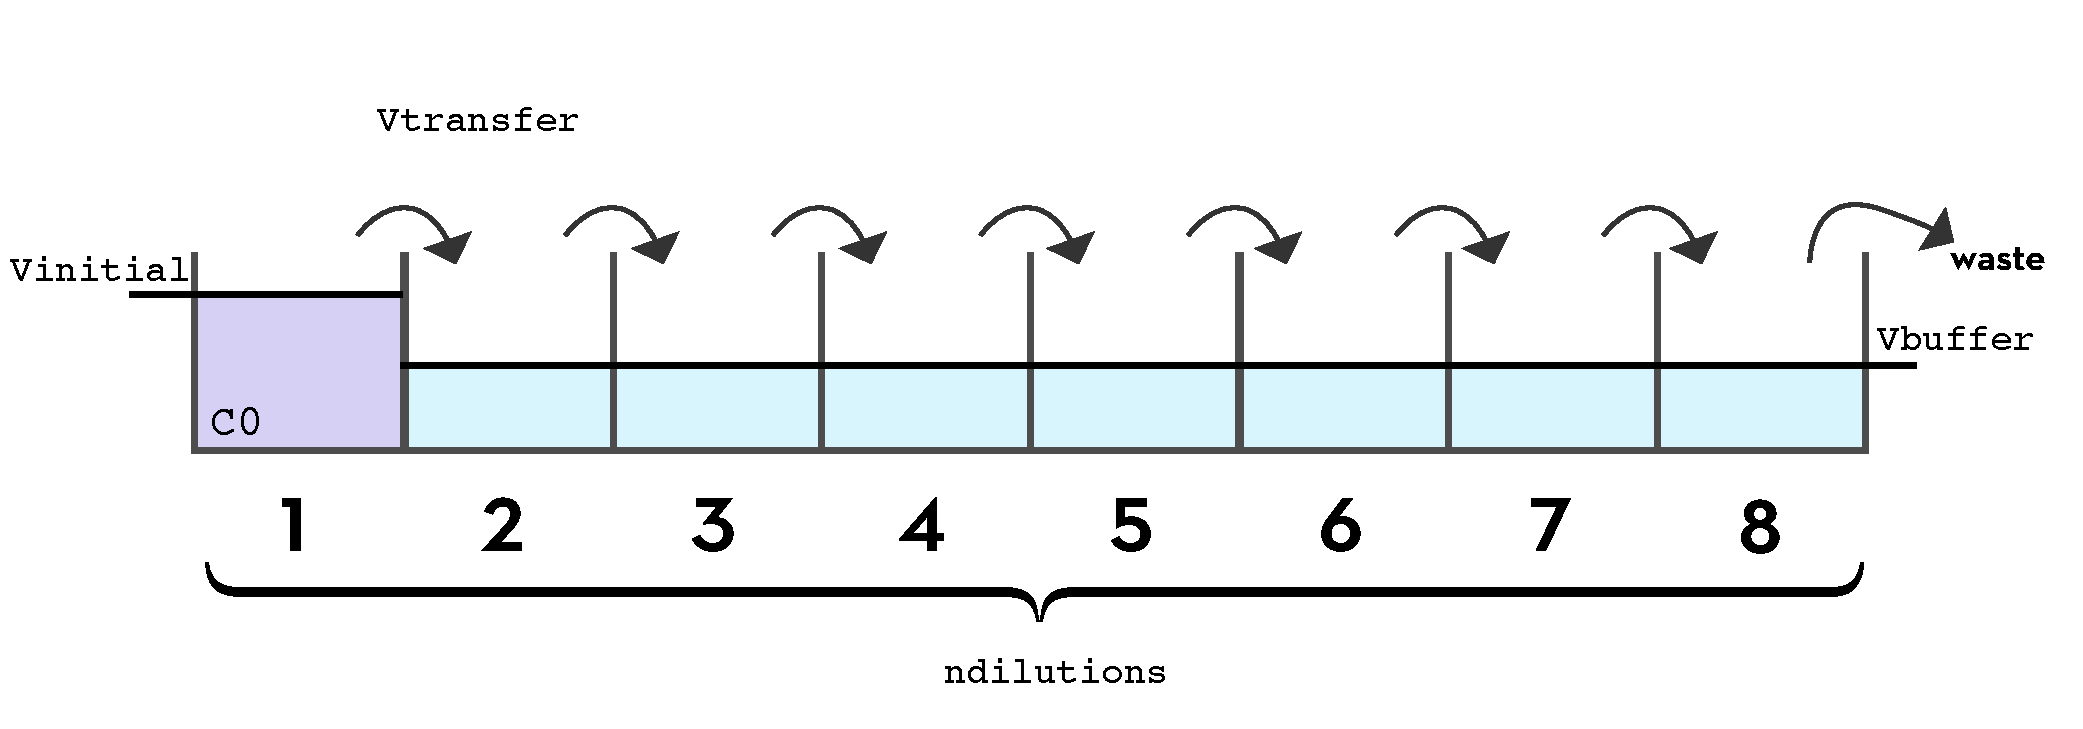
\includegraphics[width=0.5\textwidth]{../figures/dilution.pdf}

  \caption{{\bf A programmatic tip-based dilution series.}
  In this dilution series we start with our initial well at concentration, $C0$, with initial volume, $Vinitial$. A volume, $Vtransfer$, is then transferred into a volume, $Vbuffer$, of buffer. 
  In this case $Vtransfer$ and $Vbuffer$ are equal, so the concentration of the second well will be $C0/2$. This transfer is then repeated for all subsequent wells, the number of which is defined by $ndilutions$. 
  From the last well the volume $Vtransfer$ is removed, so that all wells have the same final volume of $Vtransfer=Vbuffer$.
  }
  \label{fig:dilution}
\end{figure*}

\subsubsection*{Direct dispensing technologies.}

To construct a model of a dilution series we start with our initial ligand stock in DMSO at concentration, $C0$, and then transfer a volume, $dispense\_volume$, into each well (Figure~\ref{fig:direct_dispense}). 
We can add imprecision and bias to this by using manufacturer-provided values for the Labcyte Echo: the imprecision is stated as 8\% and the inaccuracy as 10\% for the volumes in question [ref]. 
The concentration of each well is determined by the volumes $dispense\_volume$ and $mix\_volume$, each of which is defined in our model as randomly drawn from a normal distribution \ref{eq:1}, where the bias and the variance that have been pulled from a linear interpolation of the provided imprecision and inaccuracy, respectively, provided by the manufacturer.
Then, applying the parametric bootstrapping model, we can get a good estimate for the errors in volumes and concentrations (Figure~\ref{fig:volumes-n-concentrations}).

\begin{figure*}[tb]
    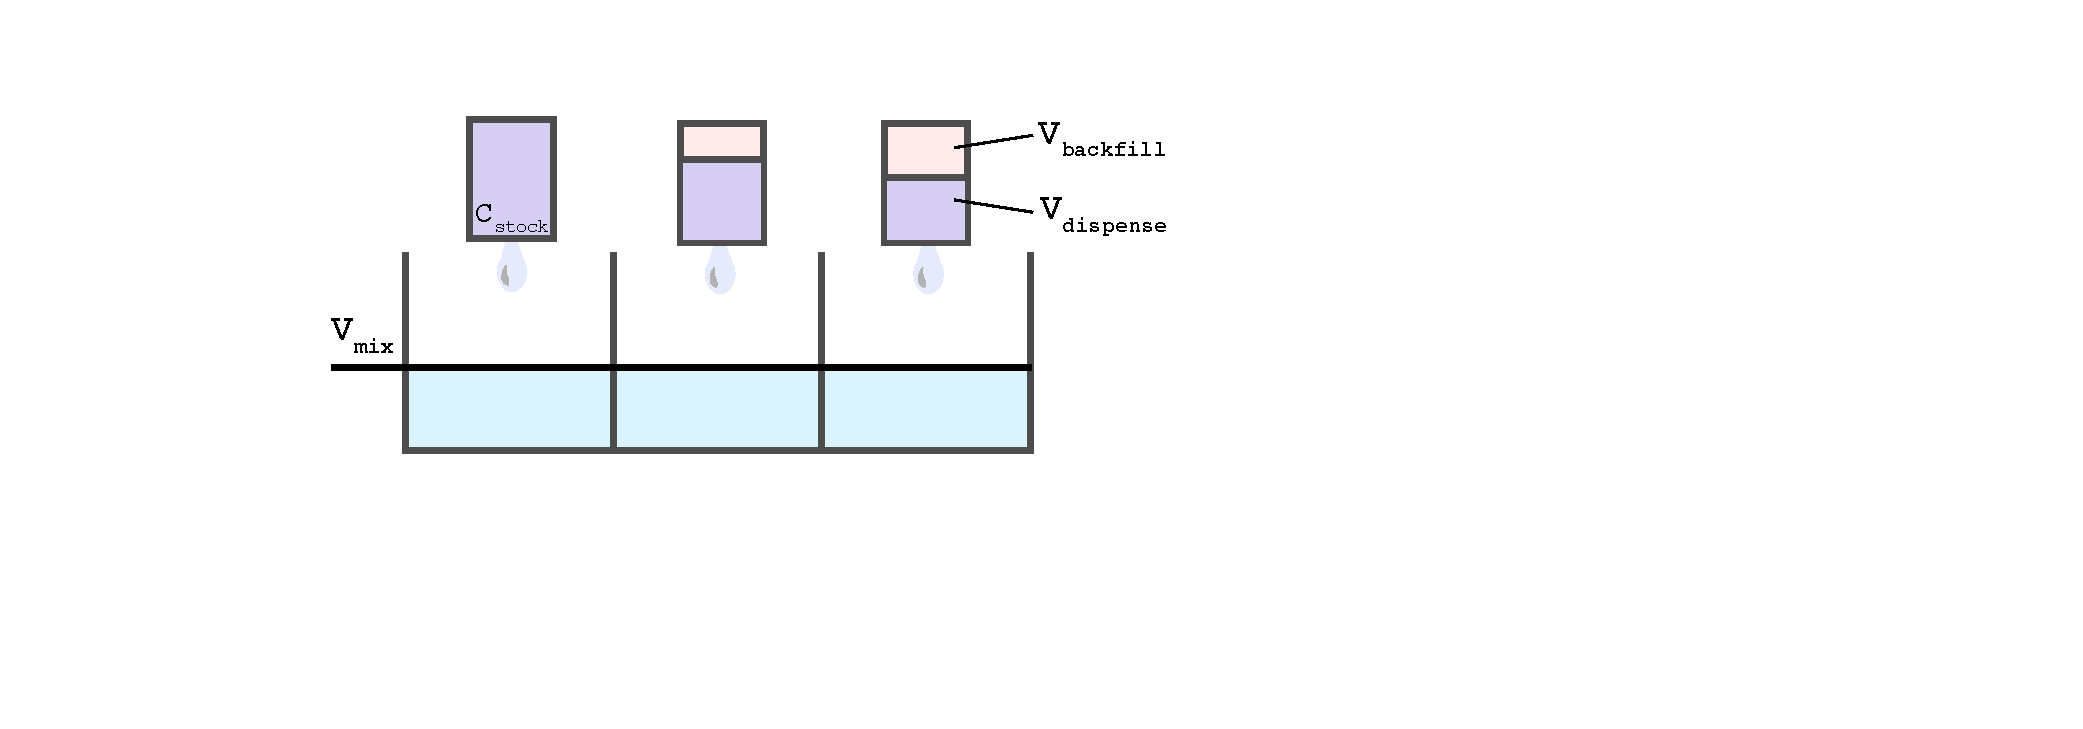
\includegraphics[trim={0 9cm 0 9cm},clip,width=0.5\textwidth]{../figures/direct_dispense.pdf}

  \caption{{\bf A programmatic direct dispense-based dilution series.}
  With direct dispense, each well is defined individually, not depending on the other, and $C0$ defines the concentration of the ligand stock. The $mix\_volume$ defines the final volume of the enzyme and ligand mix. 
  The $dispense\_volume$ is the amount of the compound stock in DMSO that is dispensed into the mix\_volume, and is what determines the final concentration of the ligand in the direct dispense assay setup. 
  To maintain a constant DMSO concentration throughout the assay, in this case 120 nL, a volume, defined by $backfill\_volume$, of pure DMSO is dispensed into the assay.
  }
  \label{ref:direct_dispense}
\end{figure*}

\subsubsection*{Fixed pipette tips and the dilution effect.}

Just including accuracy and imprecision, the errors from tip-based vs. acoustic based dispensing look quite similar, and don't seem to explain the discrepencies in the dataset in Ekins. et al. 
Another aspect of dispensing with multichannel liquid-handler, specific to liquid-based fixed-tip pipetting, such as the Tecan Genesis has, is the dilution effect. 
This dilution effect was previously characterized by a couple papers from Bristol Meyers Squibb ~\cite{dong_use_2006}~\cite{gu_dilution_2007}, where they found that the system liquid used to create the pressure differences required for pipetting, can mix with sample when it is being aspirated (Figure~\ref{fig:dilution_effect}). 
This mix of system liquid and sample dilutes the sample, and the Bristol Meyers Squibb team was able to use a combination of the Artel dye-based Multichannel Verification System (MVS) and gravimentric methods to quantify that this dilution contributes a -6.30\% inaccuracy for a target volume of 20 $\mu$L ~\cite{dong_use_2006}.
This inaccuracy can then be included in our model, using the same method of taking a random sample from a normal distribution and iterating over many replicates, and we can look at the resulting CV and bias seen in volumes, concentrations and quantities, as for the disposable tip model (which won't have this error) and the acoustic-dispensing model (Figure~\ref{fig:volumes-n-concentrations}).

\begin{figure*}[tb]
    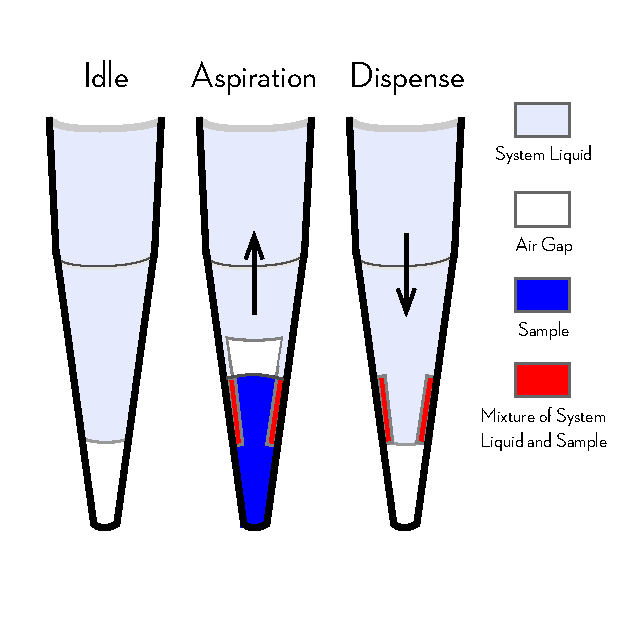
\includegraphics[width=0.325\textwidth]{../figures/dilution_effect.pdf}

  \caption{{\bf Dilution effect illustration.}
  This diagram is based on the explanation of the dilution effect from~\cite{gu_dilution_2007}. 
  A dilution effect is seen in fixed-tip automated liquid handlers that use liquid-displacement dispensing technology. 
  Aspirated sample can be diluted by the system liquid (light purple) when the liquid sticks to the side of the tip and is mixed with the sample (blue) as it is aspirated.
  This mix of system liquid and sample (red) then dilutes the sample when it is dispensed. 
  While the use of an air gap (white) reduces this dilution effect, it is still a known problem in fixed tip liquid-based automated liquid handling technologies, requiring more complex strategies to eliminate it~\cite{gu_dilution_2007}. 
  }
  \label{fig:dilution_effect}
\end{figure*}


\begin{figure*}[tb]
    
\includegraphics[width=1.0\textwidth]{../figures/placeholder.pdf}

  \caption{{\bf Comparing modeled errors in volume, concentration, and quantity for tip-based vs acoustic dispensing.}
  Using our model we can look at the variance (top) and bias (middle) in volume, concentration, and quantity as a function of the dilution.
  }
  \label{fig:volumes-n-concentrations}
\end{figure*}


\subsection*{Modeling plate reader measurement}

When measuring readouts of fluorescence assays, it is important to take intrinsic error in plate reader measurement into account. All observations have error. 
Luckily most plate readers already have these stats on hand in their manuals. 
For example the {\bf XXX} used in this example has a fluorescence detection threshold of {\bf XXX} and an error of {\bf XXX}.

\subsection*{Modeling an enzymatic reaction}

Creating a simple model of a competition assay can be done using standard formulas, here assuming we have data for $V_\mathrm{max}$. 
Similar models can be created for different assay readouts.  This is all we need to be able to understand expected variance and bias in  pIC50 values (Figure~\ref{fig:acoustic-vs-tips}).

\begin{figure*}[tb]
    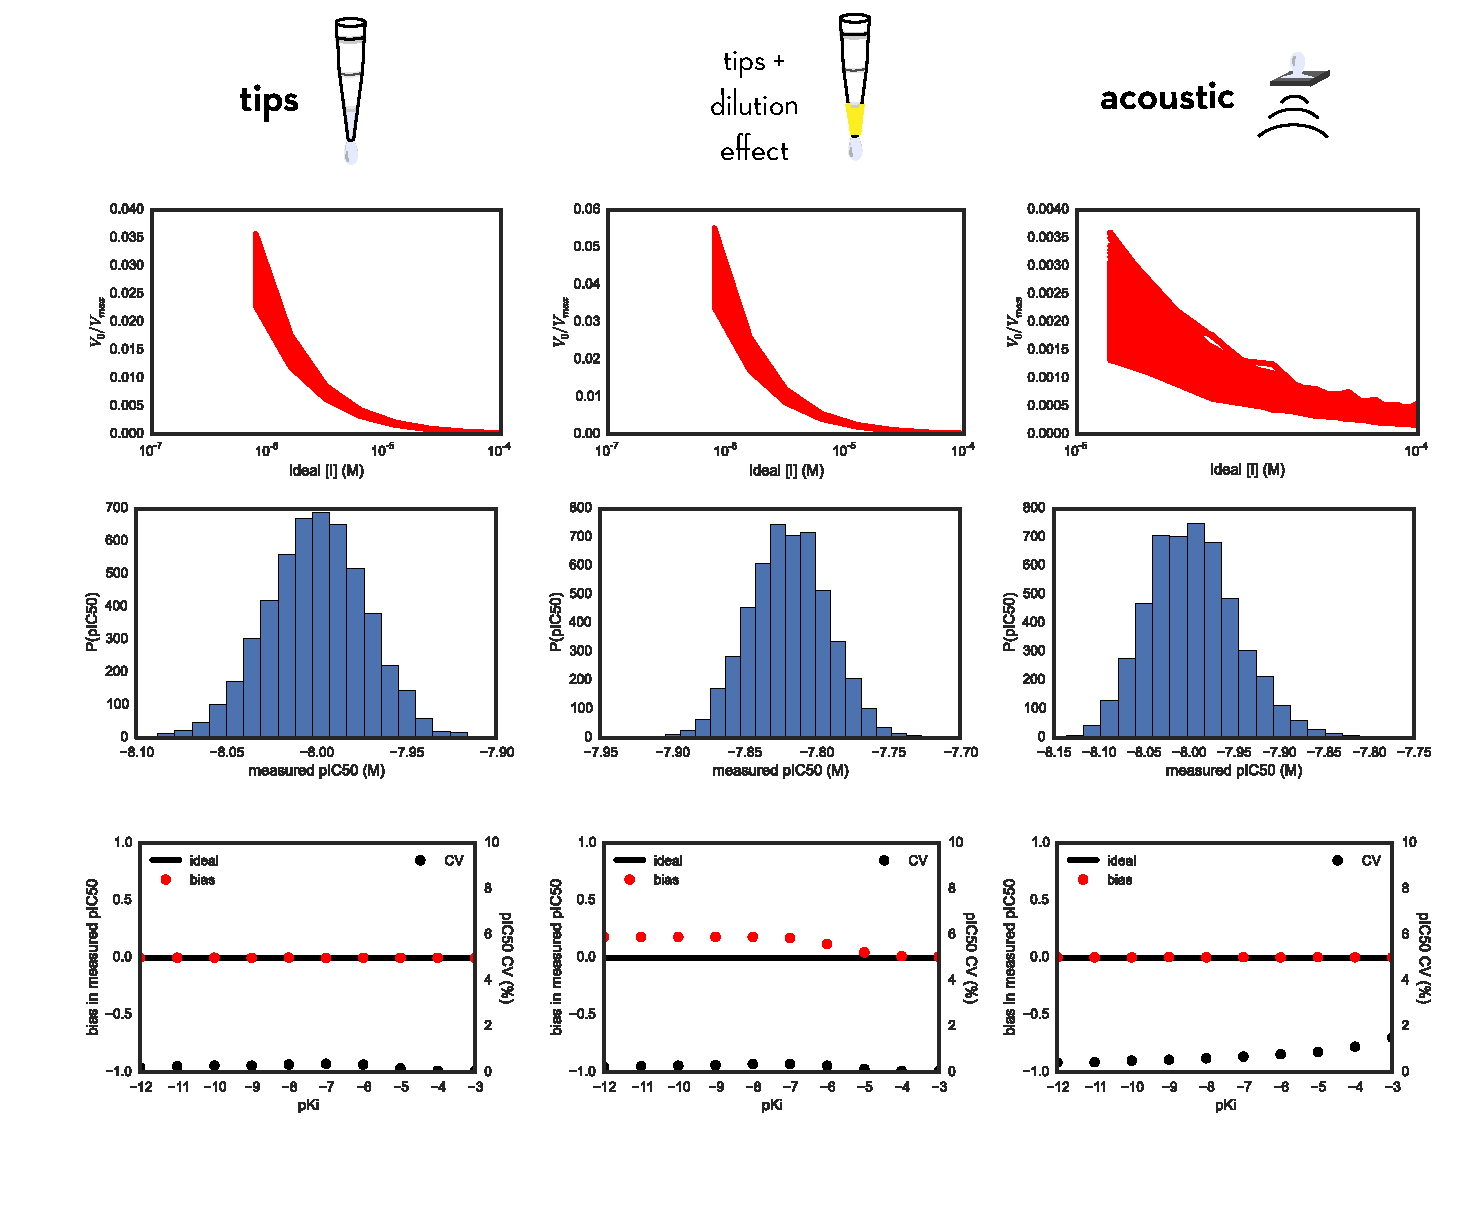
\includegraphics[width=1.0\textwidth]{../figures/tips_v_acoustic.pdf}

  \caption{{\bf Comparing modeled errors in pIC50 values from tip-based vs acoustic dispensing.}
  Using our model we can look at the variance in activity measurements as a function of inhibitor concentration $[I]$ (top), which then directly translates into a distribution of measured $pIC50$ values (middle), from which we can find out the bias and variance, or CV, as a function of pKi seen in these assays (bottom). While using acoustic dispensing methods the CV creeps up as a function of pKi, when a known dilution effect is added to the tip-based dispensing, a large bias is easy to spot.
  }
  \label{fig:acoustic-vs-tips}
\end{figure*}

\subsection*{Imprecision is insufficient to explain the Ekins discrepancy}

Plotting the inaccuracies and imprecisions and how they differ for tip-based dispensing vs. direct dispensing is extremely useful, and allows us to understand the errors in our assay results a bit better. 
It is easy to see that simple difference in these values, even when including the compounded error of the dilution series, does not give us much insight into the striking differences seen in Ekins et al between tip-based and direct dispensing.

However, if we incorporate the final component of error in tip-based dispensing, the dilution effect, we can see that correcting for this bias in plotting IC50 shifts tip-based values more toward direct-dispensing derived values (Figure~\ref{IC50_bias}).

\begin{figure*}[tb]
    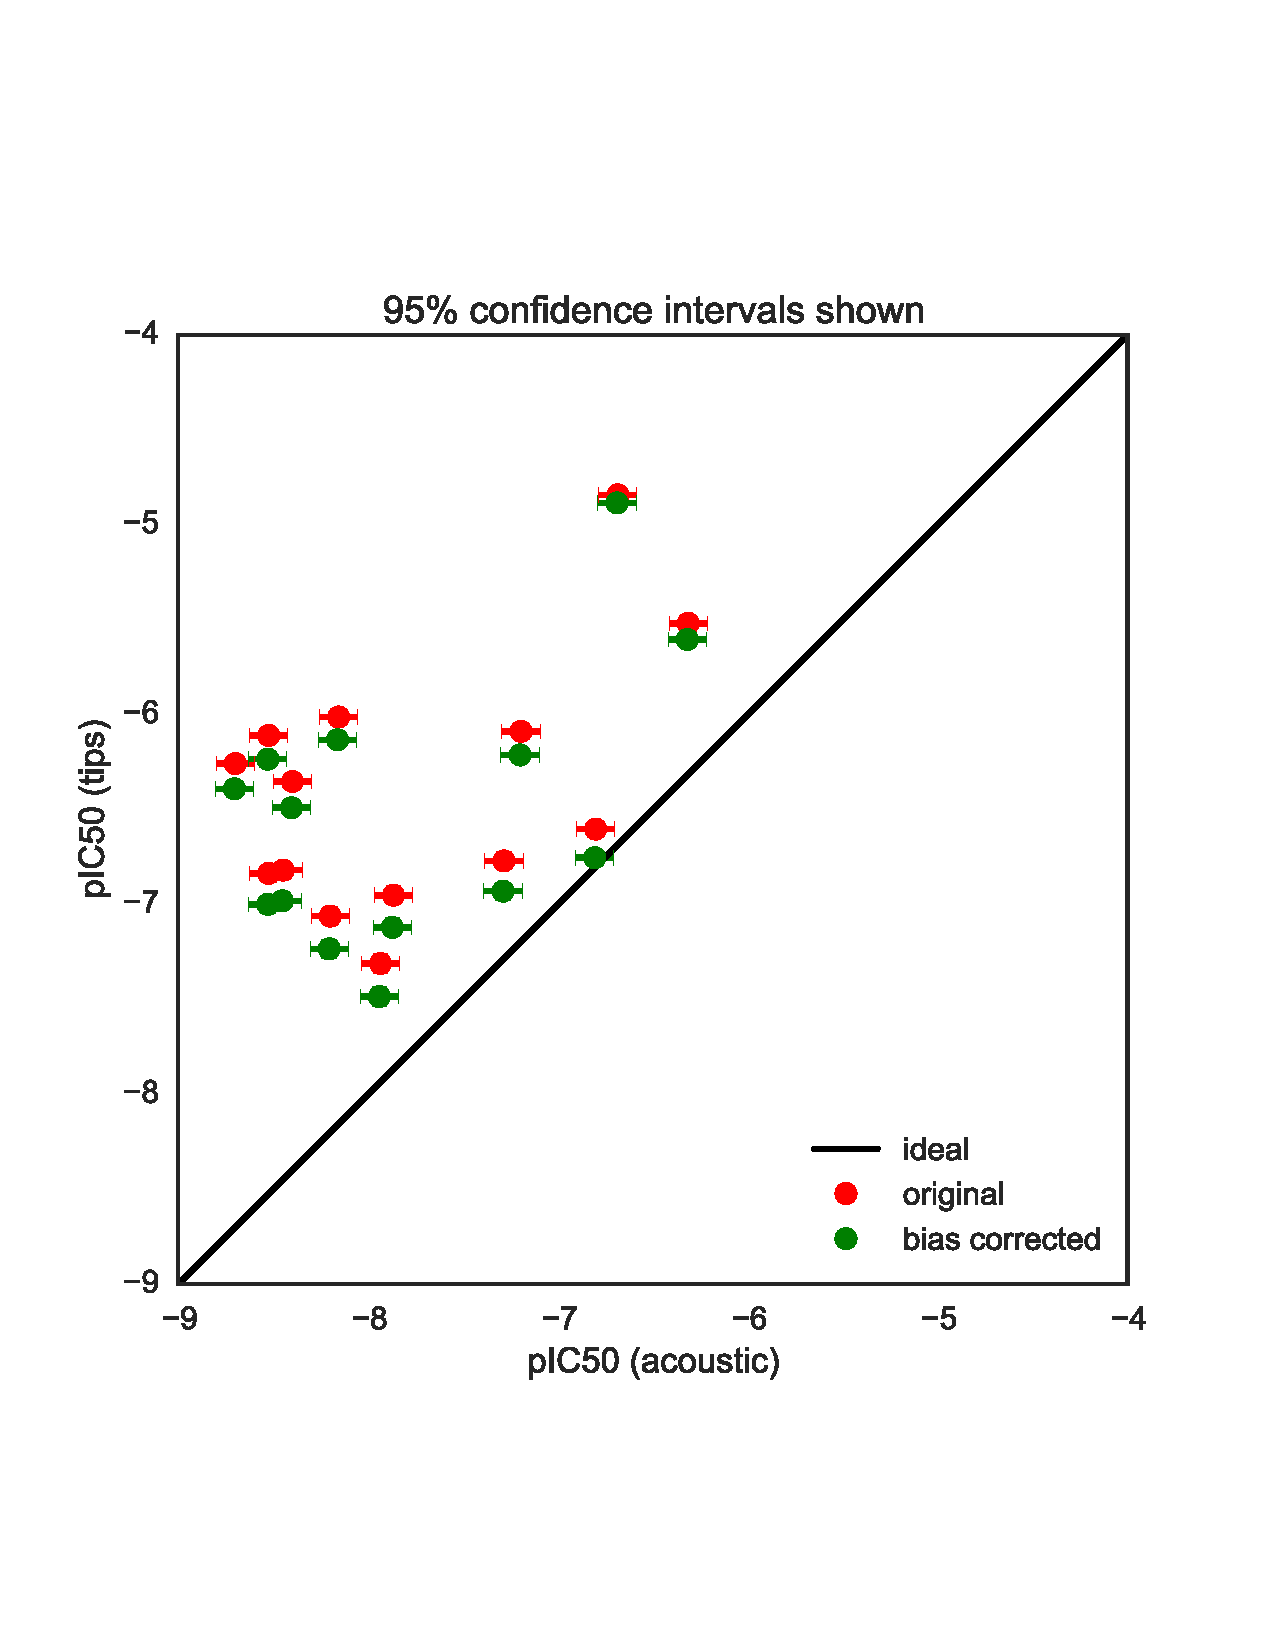
\includegraphics[trim={0 4cm 0 4cm},clip,width=0.5\textwidth]{../figures/compare-pIC50-bias_corrected.pdf}

  \caption{{\bf Adding bias shifts pIC50 values closer to equivalence.}
  Here we see (in red) the original experimental data points with errors bars representing the uncertainty calculated from our models. Adding in the bias from our models (in green) shifts the experimental pIC50 values closer to if tip-based assay and acoustic-based assay measurements resulted in the same final measurement. While this does not entirely explain the discrepancies between the two sets of data, it provides an initial insight, and shows the power of building simple error models to improve our understanding of experimental data sets.
  }
  \label{fig:IC50_bias}
\end{figure*}

%%%%%%%%%%%%%%%%%%%%%%%%%%%%%%%%%%%%%%%%%%%%%%%%%%%%%%%%%%%%%%%%%%%%%%%%%%%%%%%%%%%%%%%%%%%%%%%%%%%%%
% DISCUSSION
%%%%%%%%%%%%%%%%%%%%%%%%%%%%%%%%%%%%%%%%%%%%%%%%%%%%%%%%%%%%%%%%%%%%%%%%%%%%%%%%%%%%%%%%%%%%%%%%%%%%%
\section{Discussion}

Serial dilutions are commonly used in the process of determining biologically and clinically relevant values such as inhibition concentrations (IC$_{ 50}$)  and dissociation constants (K$_{d}$). 
While high-throughput automation methods can improve the reproducibility of these measurements over manual pipetting, even robotic liquid handlers are victim to systematic error. 
Here, we have demonstrated how a simple model {\color{red} [which, in addition to blank blank, other resources for modeling error]} that allowed us to estimate the imprecision and inaccuracy of the measured IC$_{50}$ values, as well as identify the difficulty in creating an accurate dilution series as the major contribution to discrepancies in measurements between fixed pipette tip and direct dispensing technologies. 
We hope this will be a useful tool for experimental and computational chemists to understand common sources of error within assays that use dilution series and how to model and correct for them.

This however, is just one example of what can generally be done if this model is pursued for other times of experiments relevant to computational modelers.
Ideally, experimentalists should verify ahead of time via this or a similar approach that their assay appropriately discriminates among the properties of the molecules in question given the expected range of IC$_{ 50}$s or K$_{d}$s to be probed, combined with the errors already known to be intrinsic to the experiment. 
This kind of modeling will allow for assays to even be fine tuned to make sure the data is appropriate to the question at hand. 
For example, in our own laboratory, it has informed the decision to use only direct dispensing technologies for a our fluorescent ligand-binding assays.

Not only is this sort of modeling approach useful for design ahead of time and analysis after the fact of experiments, but it can be extremely useful in determining the right tests and controls to use to be sure errors and biases are properly taken into account in general. If one is not certain about the primary sources of error in an experiment, one is arguably not certain about the results of the experiment in general. 
Understanding these errors, and being certain they are accounted for via clear benchmarks in experimental assays could help ensure the reproducibility of assays in the future, which is currently a topic of great interest. 
Especially with such a wide ranging set of assays that use dilution series, most notably toward the development of proteins and small molecules to study and treat disease, this is a very important category of experiments to understand how to make more clearly reproducible and interpretable.

While here we have illustrated the importance of modeling to the specific case of liquid handling with fixed tips in the context of measuring IC50 values for EPHB4 inhibitors, there are still large discrepancies that have not been explained, and large swaths of systems both biological and mechanical that are still open for further investigation. 
As experiments become more automated and analysis becomes more quantitative understanding these errors will be increasingly important both for the consumers (modelers) and producers (experimentalists) of these data.


%%%%%%%%%%%%%%%%%%%%%%%%%%%%%%%%%%%%%%%%%%%%%%%%%%%%%%%%%%%%%%%%%%%%%%%%%%%%%%%%%%%%%%%%%%%%%%%%%%%%%
% ACKNOWLEDGMENTS
%%%%%%%%%%%%%%%%%%%%%%%%%%%%%%%%%%%%%%%%%%%%%%%%%%%%%%%%%%%%%%%%%%%%%%%%%%%%%%%%%%%%%%%%%%%%%%%%%%%%%
\section{Acknowledgments}
\label{section:acknowledgments}

Thanks to everybody!

\begin{itemize}
  \item Cosma Shalizi for his excellent GRC talk on the bootstrap principle
  \item Funding sources (SKI, NIH core grant for JDC)
  \item Adrienne Chow, Anthony Lozada, and Tecan?
  \item Terry Stouch (JCAMD, for tireless encouragement)
  \item Anthony Nicholls (statistics of drug discovery GRC)
  \item Paul Czodrowski (for introducing us to IPython notebooks)
\end{itemize}

%%%%%%%%%%%%%%%%%%%%%%%%%%%%%%%%%%%%%%%%%%%%%%%%%%%%%%%%%%%%%%%%%%%%%%%%%%%%%%%%%%%%%%%%%%%%%%%%%%%%%%
% BIBLIOGRAPHY
%%%%%%%%%%%%%%%%%%%%%%%%%%%%%%%%%%%%%%%%%%%%%%%%%%%%%%%%%%%%%%%%%%%%%%%%%%%%%%%%%%%%%%%%%%%%%%%%%%%%%%

\bibliographystyle{prsty} 
\bibliography{dispensing-errors.bib}


\end{document}
